\documentclass[
    a4paper,
   12pt,			% font size
   headsepline
]{report}

\usepackage[utf8]{inputenc}		% Pour afficher les caracteres internationaux
\usepackage[T1]{fontenc}			% Pour l'encodage de caracteres
\usepackage[french]{babel}


\usepackage{lmodern} % Pour changer le pack de police
\usepackage{makeidx} % For table of content
\usepackage{layout}  % For \Layout comment 

\usepackage{graphicx}   % For images 
\usepackage{subcaption} % for multiple image caption






% ========= FOR LINKS IN TABLE OF CONTENT ============= % 
\usepackage{color}      % May be necessary if you want to color links
\usepackage{hyperref}   % clickable links 
\hypersetup{
    colorlinks=true,    %set true if you want colored links
    linktoc=all,        %set to all if you want both sections and subsections linked
    linkcolor=black,    %choose some color if you want links to stand out
}

\usepackage{float}      %used for figure placement with H as a parameter
\usepackage{setspace}
\usepackage{enumerate}  %like itemize but  with numbers %didnt use it yet

\usepackage[font=small,labelfont=bf]{caption}
\def\figurename{\textbf{Figure }}

%------- stuff i did not use yet -----%
\usepackage{wrapfig} %pour que je mets la photo next to the text
\usepackage{fancyhdr}
%\usepackage{tabu}
%\usepackage[final]{pdfpages}        % To Include PDFs
%------------------------------------%

\title{Projet Fin Etude}
\author{Benzerga Malek}
\date{\today}

%------------ pour le title head ------------%
\pagestyle{fancy}
\fancyhf{}
%%\rhead{Overleaf}
\lhead{Traitement,Analyse de Donnèes pour l'Evaluation de la Qualitè de la Route}
%%\rfoot{Page \thepage} pour afficher page + nombre de page
%--------------------------------------------%


% Bibliography 
%\usepackage[backend=bibtex,sorting=none]{biblatex}
%\addbibresource{bibliographie}



\begin{document}

% For that english quote %
\begin{center}
    \textit{\textbf{{\LARGE "The importance of the road infrastructure for the society could be compared with importance of blood vessels for human"}}}
    \end{center}
    \begin{flushright}
    \textit{\textbf{-A wise man.}}
    \end{flushright}
% End of that english quote %

\tableofcontents
\chapter*{Introduction générale}
\renewcommand{\thesection}{\arabic{section}}
		
 \addcontentsline{toc}{chapter}{Introduction générale}



\label{chapitre1}
		
		
\includegraphics [width=1 \linewidth, height=0.8\textheight, keepaspectratio] {Images/chapterFigures/chOne.png}
		
	
		
    \newpage
    \thispagestyle{plain}
Selon le centre national de prévention et de sécurité routière algérien :
plus de 3.049 personnes avaient trouvé la mort et 29.095 personnes avaient été blessées
dans 21.109 accidents enregistrés au niveau national lors des onze premiers mois de l'année 2019  \cite{nassimaAccidentsRouteAlger}.
\begin{figure}[h!]
  \center
  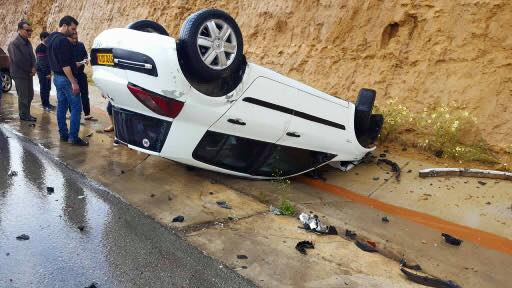
\includegraphics[width=0.75\textwidth]{Images/chapter1/accident.jpg}
  \caption{Accident de route.}
  \label{fig:Accident}
\end{figure}
Dans un scénario réel, la règle dit que plus la surface de la route est confrontée
à des changements de climat (entre le froid et le chaud) et avec un manque de soins,
plus elle subit des dégâts et affecte ensuite la vie des gens.

La surveillance de la surface des routes est un problème difficile dans le domaine des
infrastructures de transport routier dans le monde entier. Une zone en mauvais état peut
endommager les véhicules, les conducteurs et même provoquer un accident.
Au regard d'autre pays étrangés, ils sont également à l'origine de poursuites et de dommages-intérêts coûteux, par exemple,
en 2005, l'État du Michigan avait déposé plus de 7,500 réclamations pour dommages liés
aux nids-de-poule \footnote{http://www.detnews.com/2005/specialreport/0510/18/A01-350197.htm}, et les
compagnies d'assurance recevaient plus de 500,000 réclamations pour nids-de-poule chaque
année\footnote{http://www.wktv.com/special/6733696.html}.

Les municipalités du monde entier dépensent des millions de dollars pour entretenir et réparer leurs routes.
Malgré cet investissement, peu de gens sont satisfaits de la qualité de la route où ils vivent ou travaillent, car c'est  toujours trop tard!!

\section{Problématique}
De ce qui précède, l'entretien et la maintenance de la qualité de l'infrastructure routière est d'une importance vitale pour la société.

En Algérie, particulièrement, ce domaine est presque négligé, les routes endommagées sont plus nombreuses que les routes sûres.
L'entretien de la route en Algérie  passe par plusieurs phases :

\renewcommand{\labelitemi}{$\bullet$}
\begin{itemize}
  \item Détection des dégradations.
  \item Localisation des dégradations : les agents du service de contrôle de la route utilisent les points kilométriques 'PK'. pour localiser les dégradations.
  \item L'entretien de la route se fait soit par la Direction des Travaux Publics 'DTP' ou une entreprise désignée par le Ministère des Travaux Publics 'MTP'.
\end{itemize}

La détection des dégradations jusqu'à présent se fait par constatation visuelle par des agents d'entretien de la DTP, cette étape est fastidieuse et longue nécessitant un savoir-faire particulier et une expérience dans le domaine. Par conséquent les dégradations (nids-de-poule/bosses) prennent beaucoup de temps pour être réparées et par conséquent elles causeront plus de dégâts.

\section{Anomalies dans une route}
Dans nos recherches lors de l'étude de cette problématique, nous observons que les anomalies
les plus courantes sont les nids-de-poule (potholes) et les bosses (bumps).
Ces deux catégories peuvent classer la plupart des anomalies trouvées dans notre vie quotidienne.

\subsection{Les fissures}
La fissuration est une dégradation majeure qui touche l'ensemble des chaussées avec différentes origines et différents mécanismes de développement. Elle est à la source d'une accélération des dégradations propres à chaque type de chaussée par la diminution de la portance du support lors de l'infiltration d'eau et par la perte des conditions mécaniques nécessaires au maintien de la résistance des matériaux \cite{FissurationOrnierageProblematiques}.

\begin{figure}[h!]
  \center
  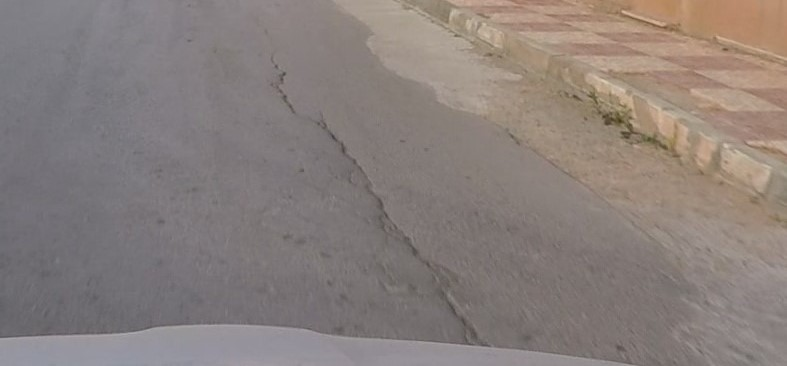
\includegraphics[width=0.75\textwidth]{Images/chapter1/fissures.jpg}
  \caption{Une fissure -Oran.}
  \label{fig:Technologies}
\end{figure}


\textbf{Causes probables :}
\renewcommand{\labelitemi}{$\bullet$}
\begin{itemize}

  \item Mauvaise construction du joint longitudinal entre deux bandes d'enrobés.
  \item Fatigue de la chaussée due à une structure insuffisante vis-à-vis du trafic
        ou une portance, du sol support insuffisante.
  \item Les caractéristiques du sol : tassement, retrait du sol argileux à la suite
        d'une longue période de sécheresse (Assèchement).
\end{itemize}


\subsection{les nids-de-poule}

Les nids-de-poule sont principalement causés par une mauvaise qualité de la chaussée ou des problèmes sous la surface.

\begin{figure}[h!]
  \center
  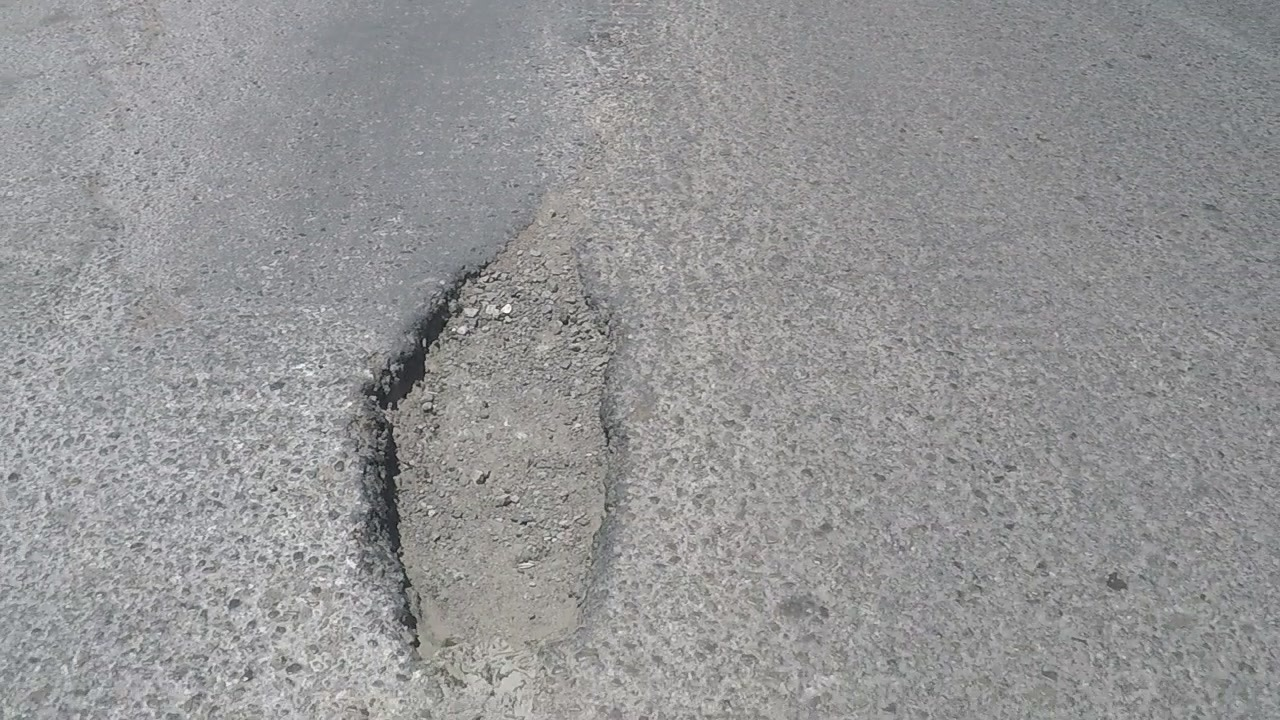
\includegraphics[width=0.75\textwidth]{Images/chapter1/Pothole.jpg}
  \caption{Nid-de-poule -Oran.}
\end{figure}

Un nid-de-poule est une dépression dans la surface d'une route, généralement une chaussée asphaltée, où la circulation
a enlevé des morceaux cassés de la chaussée.
C'est généralement le résultat de l'eau dans la structure du sol sous-jacente et du trafic passant sur la zone affectée.
L'eau affaiblit d'abord le sol sous-jacent; le trafic fatigue et brise la surface asphaltée mal supportée de la zone touchée.
L'action continue de la circulation éjecte l'asphalte et le sol sous-jacent pour créer un trou dans la chaussée.
\footnote{https://en.wikipedia.org/wiki/Pothole}



\subsection{Les Ralentisseurs (longs et courts)}

Normalement fabriquées par l'homme et généralement utilisées pour ralentir les véhicules à proximité des passages pour piétons.

On constate le plus souvent qu'ils imposent une limite de vitesse basse, inférieure à 40 km/h ou moins poussant les conducteurs à freiner d'avance.
Les ralentisseurs en général ne sont pas des anomalies, mais les ralentisseurs mal faits ou ceux qui ont été exposés à des dégâts sans réparation sont considérés comme des anomalies.
De plus, leur utilisation est parfois controversée car:

\begin{figure}[h!]
  \center
  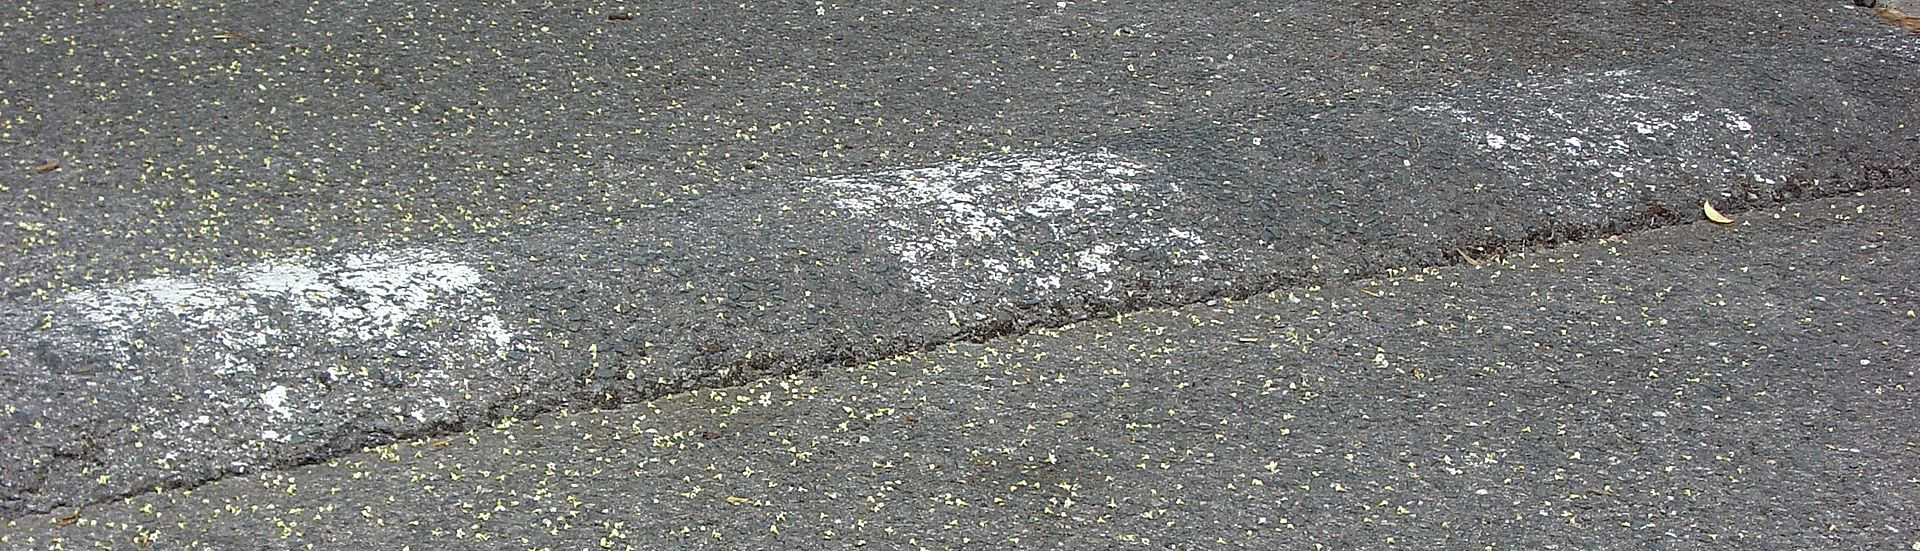
\includegraphics[width=0.75\textwidth]{Images/chapter1/Speedbump.jpg}
  \caption{Ralentisseurs -Mostaganem.}
\end{figure}
\renewcommand{\labelitemi}{$\bullet$}
\begin{itemize}
  \item Ils peuvent augmenter le bruit de la circulation.
  \item Peuvent endommager les véhicules s'ils sont traversés à une vitesse trop élevée et ralentir les véhicules d'urgence.
  \item Poussent le conducteur sur à freiner puis accélèrer, ce qui augmente considérablement la libération de gaz nocifs.
  \item Les ralentisseurs mal conçus qui se tiennent trop haut ou avec un angle
        trop aigu peuvent perturber les conducteurs et peuvent être difficiles à naviguer pour les véhicules à faible garde au sol,
        même à très basse vitesse. De nombreuses voitures de sport ont ce problème avec de tels ralentisseurs.
  \item Les ralentisseurs peuvent également présenter de graves dangers pour les motocyclistes et les cyclistes s'ils ne sont pas clairement visibles.
\end{itemize}

Les ralentisseurs coûtent entre 50 et 200 Dollar et peuvent devoir être remplacés au fil du temps
en raison de l'usure \cite{SpeedBump2020}.



\section{Objectifs et analyse des besoins}

Détecter les anomalies d'une route présente un vrai défi. Avant de commencer le projet,
nous sommes amenés à répondre aux questions suivantes :
\renewcommand{\labelitemi}{$\bullet$}
\begin{itemize}
  \item Quels sont les différents caractéristiques d'une anomalie?
  \item Quels sont les différentes difficultés et critères à prendre en compte pour décider si une anomalie est présente?
  \item Peut-on offrir une solution informatique évoluée pour assister à cette décision? Si oui :
        \begin{itemize}
          \item Comment mesurer le niveau de qualité d'une route?
          \item Comment détecter/révéler les différentes causes d'une mauvaise route?
          \item Comment localiser géographiquement chaque anomalie?
          \item Comment présenter cette solution aux services concernés de manière simple et efficace ?
        \end{itemize}
\end{itemize}

\section{Avantages}
Développer un outil de détection automatique de qualité de la route aurait pour apport:
\renewcommand{\labelitemi}{$\bullet$}
\begin{itemize}
  \item Un gain considérable de temps, efforts humains et une réduction de dépenses.
  \item Une surface de route solide et surtout sans danger pour les piétons et les conducteurs.
  \item Une meilleure circulation en ville en diminuant le nombre d'accidents de route et ainsi réduire les dégâts sur les véhicules.
\end{itemize}


\section{Solution proposée}
Nous proposons un outil permettant de :
\renewcommand{\labelitemi}{$\bullet$}
\begin{itemize}
  \item Fournir à la direction des travaux public "DTP" un moyen de se renseigner en temps réel sur la qualité des routes afin d'intervenir efficacement et le plus rapidement possible dans les travaux d'entretien. Ceci permettra d'améliorer les manques cités plus haut.
  \item Mieux assister le conducteur dans sa conduite en l'alertant  sur la qualité de la route, afin qu'il adapte sa conduite en fonction.
\end{itemize}

Pour cela, nous visons à développer un système qui proposera les fonctionnalités suivantes :
\renewcommand{\labelitemi}{$\bullet$}
\begin{itemize}
  \item Détecter les événements (les nids-de-poule et les ralentisseurs dans notre cas) en temps réel. La collecte de données brutes pour un post-traitement hors ligne.
  \item Utiliser un smartphone basé sur Android-OS avec des capteurs accéléromètres comme plate-forme matérielle / logicielle.
  \item Pouvoir fonctionner sur différents modèles de smartphones avec différents paramètres. Au cours du processus de mise en œuvre du système, l'ensemble des paramètres minimaux du smartphone doit être déterminé et décrit.
  \item Détecter les événements lors de la conduite dans différents types de véhicules à quatre roues tels que des voitures particulières, des mini-fourgonnettes et des bus. Les véhicules à deux roues tels que les motos et les scooters ne sont pas pris en compte.
\end{itemize}


\renewcommand{\thesection}{\thechapter.\arabic{section}}















\bibliographystyle{abbrv}
\bibliography{bibliographie}
%\printbibliography[heading=bibintoc]
\end{document}